% !TEX root =  master.tex
\chapter{Grundlagen}
In diesem Kapitel werden die theoretischen Grundlagen und Gedanken für die Umsetzung in Kapitel \ref{chap:Implementation} vorgestellt. Die Lösung und das Vorgehen basieren maßgeblich auf dem Beitrag \afz{\MaxLink{https://www.youtube.com/watch?v=YI1WqYKHi78}{Why is this Puzzle Impossible? - Numberphile}} von Herrn Steven Bradlow zur Lösbarkeit des \afz{14-15 puzzles} auf dem Youtube Kanal \afz{Numberphile} \autocite{Unsolvable-14-15-Numberphile-YT:online}.%
%
\section{Puzzle zu Listen wandeln} % (fold)
\label{sec:PuzzleToList}
Der Lösungsansatz aus \autocite{Unsolvable-14-15-Numberphile-YT:online} basiert auf Permutationen. Um 4x4 Puzzle besser auf Permutationen untersuchen zu können, werden die Puzzle als Listen von Zahlen dargestellt. Dazu werden die Inhalte der Zellen des Puzzle zeilenweise hintereinander in eine Liste geschrieben. Die Leerstelle, auch als \afz{blank} beschrieben, wird dabei als Zahl \afz{0} interpretiert.
Der Zustand des Puzzle aus Abb.\ref{fig:Perm_puzzle_start_Pic}
\begin{figure}[H]
	\centering
	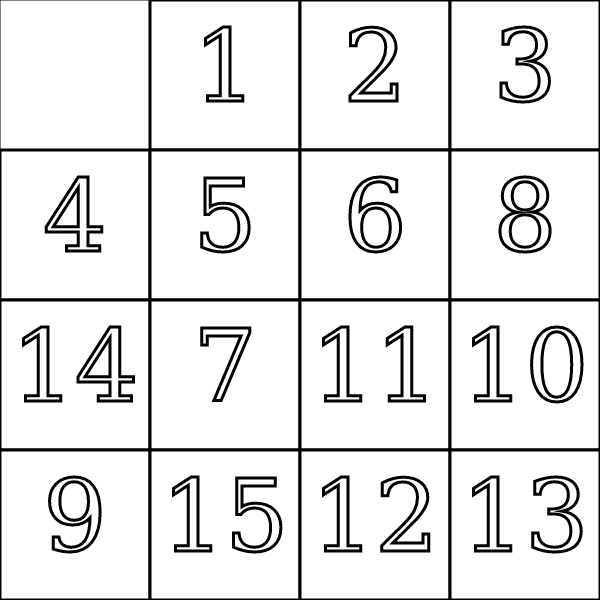
\includegraphics[width=.5\textwidth,keepaspectratio]{img/Start_Puzzle2.png}
	\captionsetup{format=hang}
	\caption{Beispiel Zustand eines 4x4-Puzzle \label{fig:Perm_puzzle_start_Pic}}
\end{figure}
\begin{minipage}{\linewidth}
	wird als Liste aus Zahlen wie folgt dargestellt:
	\begin{center}
		$State = \{0,1,2,3,4,5,6,8,14,7,11,10,9,15,12,13\}$
	\end{center}
\end{minipage}\WNL%
Wichtig ist bei der Betrachtung der lösbaren Puzzle und des Vorgehens der Lösung aus \autocite{Unsolvable-14-15-Numberphile-YT:online} aber auch anderer verfügbarer Quellen \autocite{solving-15-puzzle-lvi:article,geeksforgeeks:online,archer-15-puzzle:article}, dass die Bezeichnung der Leerstelle oder die Art der Konvertierung eines Puzzle zu einer Liste variiert. Die meisten Lösungen sehen den Zielzustand aus Abb.\ref{fig:Perm_puzzle_end_allOther} vor, wobei die Leerstelle dann die Nummer \afz{16} trägt. Um mit den Darstellungen von Herrn Stroetmann aus dem Vorlesungsskript \autocite{github-stroetmann:online} übereinzustimmen, wird der Zielzustand aus Abb.\ref{fig:Perm_puzzle_end_stroet} angestrebt, bei dem die Leerstelle die Nummer \afz{0} trägt.\\
%
\begin{minipage}{\linewidth}
	\begin{minipage}[t]{0.45\linewidth}
		\begin{figure}[H]
			\centering
			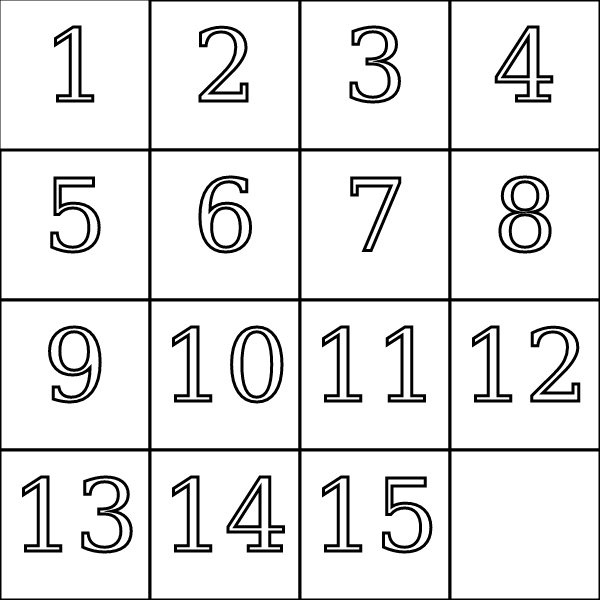
\includegraphics[width=\linewidth,keepaspectratio]{img/End_Puzzle_AO.png}
			\captionsetup{format=plain, indention=0pt}
			\caption{Häufig verwendeter Zielzustand eines 4x4-Puzzle \label{fig:Perm_puzzle_end_allOther}}
		\end{figure}
	\end{minipage}
	\hfill
	\begin{minipage}[t]{0.45\linewidth}
		\begin{figure}[H]
			\centering
			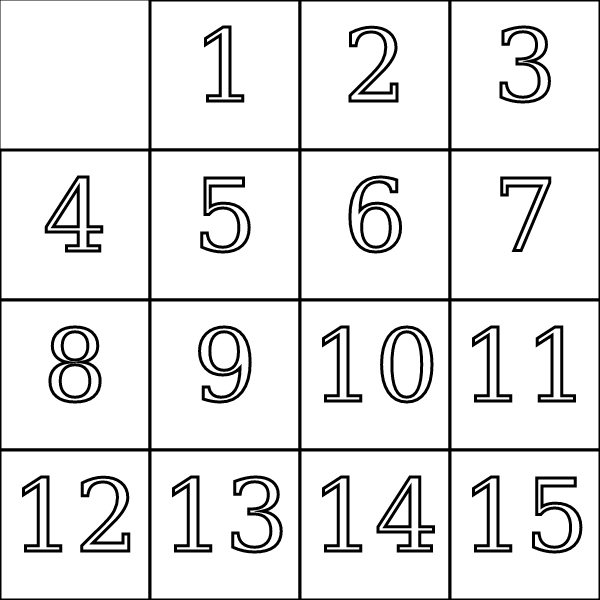
\includegraphics[width=\linewidth,keepaspectratio]{img/End_Puzzle_Stroetmann.png}
			\captionsetup{format=plain, indention=0pt}
			\caption{\label{fig:Perm_puzzle_end_stroet}Verwendeter Zielzustand eines 4x4-Puzzles aus dem Skript von Herrn Stroetmann \autocite{github-stroetmann:online}}
		\end{figure}
	\end{minipage}
\end{minipage}\WNL%

\section{Zustände als Permutationen} % (fold)
\label{sec:Permutation}
Die Grund-Idee der Lösbarkeitsüberprüfung von Bradlow basiert auf dem Vergleichen der Paritäten zwischen benötigten Transpositionen und benötigter Züge zum Verrücken der Leerstelle. Im Folgenden wird die Idee aus seinem Beitrag \autocite{Unsolvable-14-15-Numberphile-YT:online} zusammengefasst vorgestellt.\WNL

Die Vorstellung des Verfahrens beginnt Bradlow damit die Puzzle wie in der vorherigen Sektion in Zahlen Reihen zu wandeln. Durch das Vertauschen von 2 beliebigen Zahlen aus dieser Zahlenreihe entsteht eine Permutation der vorherigen Reihe. Auf diese Weise sei jeder möglicher Zustand in dem sich das Puzzle befinden kann als eine Permutation einer zugrundeliegenden aufsteigend sortieren Zahlenreihe zu sehen. Für diese Permutationen beschreit er die folgenden zwei Eigenschaften:
\begin{enumerate}
	\item[\textbf{E1}] Jede dieser Permutationen lässt sich nur durch das Nutzen von Transpositionen, also dem Vertauschen von Zwei Elementen aus der Liste, während die restlichen gleich bleiben, in eine andere Permutation überführen \cite[Vgl.][7min,07sec]{Unsolvable-14-15-Numberphile-YT:online}.
	\item[\textbf{E2}] Die Anzahl der Schritte, die für das Überführen einer Permutation in eine andere Permutation mithilfe von Transpositionen benötigt wird, ist nicht Festgelegt, aber die Parität dieser Zahl ist fest \cite[Vgl.][10min,13sec]{Unsolvable-14-15-Numberphile-YT:online}.
\end{enumerate}
Basierend auf diesen Eigenschaften fährt er fort, dass die Parität der Anzahl notwendiger Transpositionen durch das zielgerichtete Tauschen der Zahlen, mit dem ziel einer aufsteigen sortieren Zahlenreihe, ermittelt werden kann. Wie in der vorherigen Sektion beschrieben, sieht auch Bradlow die sortierte Zahlenreihe
\begin{center}
	$Goal_{Bradlow} = {1,2,3,4,5,6,7,8,9,10,11,12,13,14,15,16}$
\end{center}
als Abbild des Zielzustandes vor. Daher ist in seinem Vortrag das Ziel der Transpositionen die aufsteigend sortierte Liste. Durch E1 ist sicher gestellt, dass die sortiere Liste erreicht werden kann. E2 begründet, dass die Parität der für die Sortierung notwendigen Transpositionen mit der Parität der notwendigen Züge, wenn das Puzzle lösbar ist, übereinstimmt, obwohl die Regeln des Puzzles nicht betrachtet und somit möglicherweise nicht eingehalten werden.\WNL
Im zweiten Schritt der Lösbarkeitsüberprüfung ermittelt Bradlow die Parität der notwendigen legalen Züge zum Überführen der Leerstelle aus dem Startzustand zum Zielzustand. Dabei ist ebenfalls jeder einzelne Zug als eine Transposition zu sehen.\WNL%
Lösbar ist ein Puzzle nach Bradlow dann, wenn die ermittelten Paritäten übereinstimmen. Denn nach E2 sind die Paritäten festgelegt und können nicht verändert werden. Die Parität der Leerstellen Bewegung ist Legal, während Parität der notwendigen zur Sortierung notwendigen Züge nur hypothetisch sind. stimmen die Paritäten nicht über ein existiert nach E2 keine Möglichkeit beide Ziele, also die Sortierung ebenso wie das einhalten Zugregeln einzuhalten. 
\WNL
In der nächsten Sektion wird dieses Verfahren an einem Beispiel schrittweise durchgegangen.
\WNL
Für die Sektion \ref*{cha:Umsetzung}, soll noch erwähnt werden, dass sich die Leerstelle nur horizontal und vertikal \afz{bewegen} darf und sich die Anzahl der Züge so mithilfe der Manhattan-Distanz ermitteln lässt.


\section{Nutzen des Algorithmus an Beispielen} % (fold)
\label{sec:PermutationExamples}
Aus der Vorlesung von Herrn Stroetmann und dem begleitenden Skript \autocite{github-stroetmann:online} ist bekannt, dass sich Puzzle aus Abb. \ref{fig:Ex1_start} lösen, also in den Zielzustand aus Abb. \ref{fig:Ex1_end} überführen lässt.\\
\begin{minipage}{\linewidth}
	\begin{minipage}[t]{0.45\linewidth}
		\begin{figure}[H]
			\centering
			\includegraphics[width=\linewidth,keepaspectratio]{img/Ex1_start.png}
			\captionsetup{format=plain, indention=0pt}
			\caption{Beispiel1: Startzustand eines 4x4-Puzzles nach figure 2.20 aus \autocite{github-stroetmann:online} \label{fig:Ex1_start}}
		\end{figure}
	\end{minipage}
	\hfill
	\begin{minipage}[t]{0.45\linewidth}
		\begin{figure}[H]
			\centering
			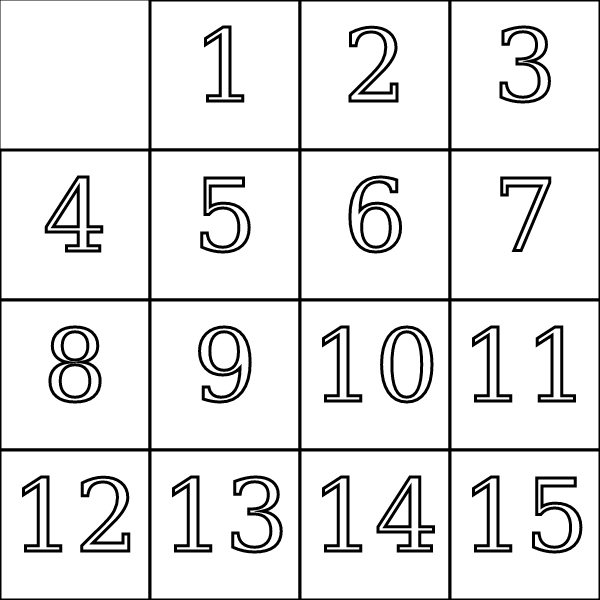
\includegraphics[width=\linewidth,keepaspectratio]{img/End_Puzzle_Stroetmann.png}
			\captionsetup{format=plain, indention=0pt}
			\caption{\label{fig:Ex1_end}Beispiel1: Zu erreichender Zielzustand für das Puzzle nach figure 2.20 aus \autocite{github-stroetmann:online}}
		\end{figure}
	\end{minipage}
\end{minipage}\\\WNL%
Der Algorithmus aus dem vorherigen Abschnitt schätzt diese Puzzles ebenfalls als lösbar ein.\\
\begin{figure}[H]
	\begin{enumerate}
		\item[\textbf{S1.1}] Konvertierung der Puzzle-Zustände in Zahlenreihen
		      \begin{align*}
			      start_{ex1} = \{0,1,2,3,4,5,6,8,14,7,11,10,9,15,12,13\} \\
			      end_{ex1} = \{0,1,2,3,4,5,6,7,8,9,10,11,12,13,14,15\}
		      \end{align*}
		\item[\textbf{S1.2}] Notwendige Transpositionen $T_{ex1}$ um $start_{ex1}$ zu sortieren:
		      \begin{align*}
			      0,1,2,3,4,5,6,8,14,7,11,10,9,15,12,13 & \hspace{20pt} (\space 8,\space 7) \\
			      0,1,2,3,4,5,6,7,14,8,11,10,9,15,12,13 & \hspace{20pt} (14,\space 8)       \\
			      0,1,2,3,4,5,6,7,8,14,11,10,9,15,12,13 & \hspace{20pt} (14,\space 9)       \\
			      0,1,2,3,4,5,6,7,8,9,11,10,14,15,12,13 & \hspace{20pt} (11,10)             \\
			      0,1,2,3,4,5,6,7,8,9,10,11,14,15,12,13 & \hspace{20pt} (14,12)             \\
			      0,1,2,3,4,5,6,7,8,9,10,11,12,15,14,13 & \hspace{20pt} (15,13)             \\
			      0,1,2,3,4,5,6,7,8,9,10,11,12,13,14,15 &
		      \end{align*}
		      \begin{align*}
			      T_{ex1} = \{(8,7),(14,8),(14,9),(11,10),(14,12),(15,13)\} \\
			      \left\vert T_{ex1}\right\vert = 6 \rightarrow \texttt{Parität} = 0
		      \end{align*}
		\item[\textbf{S1.3}] Anzahl der notwendigen Züge $z_{ex1}$ um das Leerfeld von der Postion aus dem Startzustand (Koordinaten $(0,0)$) an die Postion des Zielzustandes (Koordinaten $(0,0)$) zu verschieben.
		      \begin{align*}
			      z_{ex1} = \left | 0 - 0 \right | + \left | 0 - 0 \right | \\
			      z_{ex1} = 0 \rightarrow \texttt{Parität} = 0
		      \end{align*}
		\item[\textbf{S1.4}] Die Paritäten stimmen überein, das Puzzle \textcolor{OliveGreen}{ist lösbar}.
	\end{enumerate}
	\caption{Beispiel 1: Anwendung des Algorithmus auf ein Vorlesungsbeispiel \label{fig:Ex1_algo}}
\end{figure}
Dazu wird wie in Abb. \ref{fig:Ex1_algo} schrittweise vorgegangen. Zunächst werden, wie im Abschnitt \ref{sec:PuzzleToList} und in Schritt 1 (S1.1) dargestellt, die Zustände in Zahlenreihen konvertiert.
Anschließend werden die Paritäten ermittelt (S1.2 und S1.3). Zunächst die Parität der Anzahl notwendiger Transpositionen und anschlie"send die Parität benötigter Züge um die Leerstelle korrekt zu platzieren. Im abschlie"senden Schritt (S1.4) werden die ermittelten Paritäten verglichen. In diesem Beispiel stimmen diese Paritäten überein. Das Beispiel ist also lösbar.%
\WNL%
%
% Loyd
%
Als nächstes wird das Puzzle von Loyd aus der Einleitung betrachtet. Der bereits bekannte Startzustand ist in Abb. \ref{fig:Ex2_start} zur Vereinfachung erneut abgebildet. Der Zielzustand ist daneben in Abb. \ref{fig:Ex2_end} dargestellt.\\
\begin{minipage}{\linewidth}
	\begin{minipage}[t]{0.45\linewidth}
		\begin{figure}[H]
			\centering
			\includegraphics[width=\linewidth,keepaspectratio]{img/Ex2_start.png}
			\captionsetup{format=plain, indention=0pt}
			\caption{Beispiel2: Startzustand für das Loyd Puzzle \label{fig:Ex2_start}}
		\end{figure}
	\end{minipage}
	\hfill
	\begin{minipage}[t]{0.45\linewidth}
		\begin{figure}[H]
			\centering
			\includegraphics[width=\linewidth,keepaspectratio]{img/Ex2_end.png}
			\captionsetup{format=plain, indention=0pt}
			\caption{\label{fig:Ex2_end}Beispiel2: Zu erreichender Zielzustand für das Loyd Puzzle}
		\end{figure}
	\end{minipage}
\end{minipage}\\\WNL%
Auch hier wird der beschriebene Algorithmus angewandt, das Vorgehen ist in Abb. \ref{fig:Ex2_algo} skizziert.
\begin{figure}[H]
	\begin{enumerate}
		\item[\textbf{S2.1}] Konvertierung der Puzzle-Zustände in Zahlenreihen
		      \begin{align*}
			      start_{ex2} = \{1,2,3,4,5,6,7,8,9,10,11,12,13,15,14,0\} \\
			      end_{ex2} = \{1,2,3,4,5,6,7,8,9,10,11,12,13,14,15,0\}
		      \end{align*}
		\item[\textbf{S2.2}] Notwendige Transpositionen $T_{ex2}$ um $start_{ex2}$ zu $end_{ex2}$ zu überführen:
		      \begin{align*}
			      1,2,3,4,5,6,7,8,9,10,11,12,13,15,14,0 & \hspace{20pt} (15,14) \\
			      1,2,3,4,5,6,7,8,9,10,11,12,13,14,15,0 &
		      \end{align*}
		      \begin{align*}
			      T_{ex2} = \{(14,15)\} \\
			      \left\vert T_{ex2}\right\vert = 1 \rightarrow \texttt{Parität} = 1
		      \end{align*}
		\item[\textbf{S2.3}] Anzahl der notwendigen Züge $z_{ex2}$, um das Leerfeld von der Postion aus dem Startzustand (Koordinaten $(3,3)$) an die Postion des Zielzustandes (Koordinaten $(3,3)$) zu verschieben.
		      \begin{align*}
			      z_{ex1} = \left | 3 - 3 \right | + \left | 3 - 3 \right | \\
			      z_{ex1} = 0 \rightarrow \texttt{Parität} = 0
		      \end{align*}
		\item[\textbf{S2.4}] Die Paritäten stimmen nicht überein, das Puzzle ist somit \textcolor{red}{nicht lösbar}.
	\end{enumerate}
	\caption{Beispiel2: Anwendung des Algorithmus auf das Loyd Puzzle \label{fig:Ex2_algo}}
\end{figure}
Da die Zielzustände der beiden Puzzle verschieden sind (Abb. \ref{fig:Ex1_end} und Abb. \ref{fig:Ex2_end}), unterscheiden sich auch die Zahlenreihen als welche diese dargestellt werden. Doch zur Übersichtlichkeit wurde sowohl in S1.1 als auch in S2.1 die Leerstelle mit der Zahl \afz{0} kodiert. Es ist leicht zu erkennen, dass nur eine Transposition notwendig ist, um die Zahlenreihe $start_{ex2}$ in die Reihe $end_{ex2}$ zu überführen, die Parität des Vorgangs ist also 1. Da sich die Leerstelle bereits an der korrekten Stelle befindet, sind keine Züge notwendig, die Parität ist also 0. Da die Paritäten unterschiedlich sind, kategorisiert der Algorithmus dieses Puzzle korrekter weise als  nicht lösbar ein.\WNL
%
% endzustände
%
Die Wahl des Endzustandes ist relevant bei der Lösbarkeitsüberprüfung eines Puzzles. In der Sektion \ref{sec:Permutation} wurde explizit hervorgehoben, dass sich der in der Literatur übliche Endzustand (Abb. \ref{fig:Ex2_end}) von dem in Herrn Stroetmanns Skript \autocite{github-stroetmann:online} (Abb. \ref{fig:Ex1_end}) unterscheidet. In Abb. \ref{fig:Ex3_algo} zeigt der Algorithmus, dass diese Endzustände nicht ineinander Überführbar sind, In Schritt S3.1 werden Leerstellen erneut mit der Zahl \afz{0} kodiert.
\begin{figure}[H]
	\begin{enumerate}
		\item[\textbf{S3.1}] Konvertierung der Puzzle-Zustände in Zahlenreihen
		      \begin{align*}
			      end_{Loyd} = \{1,2,3,4,5,6,7,8,9,10,11,12,13,14,15,0\} \\
			      end_{Stroetmann} = \{0,1,2,3,4,5,6,7,8,9,10,11,12,13,14,15\}
		      \end{align*}
		\item[\textbf{S3.2}] Notwendige Transpositionen $T_{ex3}$ um $end_{Loyd}$ zu $end_{Stroetmann}$ überführen:
		      \begin{align*}
			      1,2,3,4,5,6,7,8,9,10,11,12,13,14,15,0 & \hspace{20pt} (1,0)   \\
			      0,2,3,4,5,6,7,8,9,10,11,12,13,14,15,1 & \hspace{20pt} (2,1)   \\
			      0,1,3,4,5,6,7,8,9,10,11,12,13,14,15,3 & \hspace{20pt} (3,2)   \\
			      0,1,2,4,5,6,7,8,9,10,11,12,13,14,15,3 & \hspace{20pt} (4,3)   \\
			      0,1,2,3,5,6,7,8,9,10,11,12,13,14,15,4 & \hspace{20pt} (5,4)   \\
			      0,1,2,3,4,6,7,8,9,10,11,12,13,14,15,5 & \hspace{20pt} (6,5)   \\
			      0,1,2,3,4,5,7,8,9,10,11,12,13,14,15,6 & \hspace{20pt} (7,6)   \\
			      0,1,2,3,4,5,6,8,9,10,11,12,13,14,15,7 & \hspace{20pt} (8,7)   \\
			      0,1,2,3,4,5,6,7,9,10,11,12,13,14,15,8 & \hspace{20pt} (9,8)   \\
			      0,1,2,3,4,5,6,7,8,10,11,12,13,14,15,9 & \hspace{20pt} (10,9)  \\
			      0,1,2,3,4,5,6,7,8,9,11,12,13,14,15,10 & \hspace{20pt} (11,10) \\
			      0,1,2,3,4,5,6,7,8,9,10,12,13,14,15,11 & \hspace{20pt} (12,11) \\
			      0,1,2,3,4,5,6,7,8,9,10,11,13,14,15,12 & \hspace{20pt} (13,12) \\
			      0,1,2,3,4,5,6,7,8,9,10,11,12,14,15,13 & \hspace{20pt} (14,13) \\
			      0,1,2,3,4,5,6,7,8,9,10,11,12,13,15,14 & \hspace{20pt} (15,14) \\
			      0,1,2,3,4,5,6,7,8,9,10,11,12,13,14,15
		      \end{align*}
		      \begin{align*}
			      T_{ex3} = \{(1,0),(2,1),(3,2),(4,3),(5,4),(6,5),(7,6),(8,7),(9,8),(10,9),(11,10), \\(12,11),(13,12),(14,13),(15,14)\}\\
		      \end{align*}
		      \begin{align*}
			      \left\vert T_{ex3}\right\vert = 15 \rightarrow \texttt{Parität} = 1
		      \end{align*}
		\item[\textbf{S3.3}] Anzahl der notwendigen Züge $z_{ex2}$ um das Leerfeld von der Postion aus Loyds Endzustand (Koordinaten $(3,3)$) an die Postion des Zielzustandes von Stroetmann (Koordinaten $(0,0)$) zu verschieben.
		      \begin{align*}
			      z_{ex3} = \left | 3 - 0 \right | + \left | 3 - 0 \right | \\
			      z_{ex3} = 6 \rightarrow \texttt{Parität} = 0
		      \end{align*}
		\item[\textbf{S3.4}] Die Paritäten stimmen nicht überein, das Puzzle ist somit \textcolor{red}{nicht lösbar}.
	\end{enumerate}
	\caption{Beispiel 2: Anwendung des Algorithmus auf die Überführbarkeit der Endzustände von Loyd und Stroetmann. \label{fig:Ex3_algo}}
\end{figure}
Ist ein Puzzle also für den einen Endzustand lösbar, ist es für den anderen Endzustand automatisch nicht lösbar, da es keine Möglichkeit gibt die Endzustände ineinander zu überführen.
%Endzustände

% Betrachtung eines lösbaren 4x4 Puzzles von Stroetman & Betrachtung des Loyd puzzles mit dem Algorithmus
%
% \section{Kontext Vorlesung + Abgrenzung} % (fold)
\label{cha:Kontext Vorlesung}

% chapter Kontext Vorlesung (end)% was sollte hier nochmal rein? wird das nciht pben abgegrenzt?
%
%
%
% \section{Sortieralgorithmen} % (fold)
\label{cha:Sortieralgorithmen}
Mit Ordnung?!
% chapter Sortieralgorithmen (end) % bissle OP das hier reinzu nehmen, lieber später den umgesetzten Sortier algorithmus Bubblesort erwähnen und sagen dass er halt auch nur Transpositionen macht somit nach E1 gültige Lösungen erhät und nach E2 geeigent ist die Parität zu berechnen , nachvollziehbar ist und deshlab genommen wird
%
%
% Endzustände sind nicht ineinander überführbar
%
%
% Betrachtung von 2x2 Puzzle um zu zeigen dass es immer 2pfade gibt
%hier könnten wir die Theorie dazu aufschrieben udn in Max Teil könnten wir den Test dazu implemetnieren in dme wir alle Permutationen notieren und in gruppen sortieren, jede aus der Gruppe muss mit jeder aus der gruppe erreichbar sein, und jedes aus Gruppe darf nicht von der anderen Gruppe aus erreicht werden. Das ganze dann halt über so ein assert generelles aufspalte eines Normalen und eienes Testdokumentes 
% Betrachtung des Loyd Puzzles

